\thispagestyle{fancy}
\begin{center}
	\LARGE{\textbf{El potenciómetro}}
\end{center}
\section{Objetivos}
Al finalizar esta experiencia, usted estará capacitado para:
\begin{enumerate}
	\item Conectar un potenciómetro como un divisor de tensión.
	\item Medir la tensión de salida de un potenciómetro, si está conectado como divisor de tensión, con o sin carga.
	\item Construir un gráfico de las relaciones entre la rotación del cursor del potenciómetro y la tensión de salida. 
\end{enumerate}
\section{Conocimientos previos}
Un potenciómetro posee una aguja rotativa que hace contacto con una resistencia.
\begin{figure}[h]
	\centering
	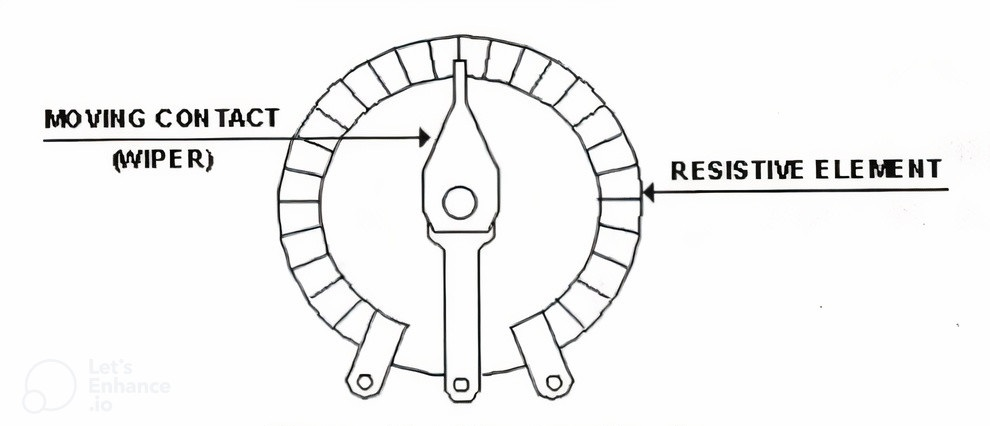
\includegraphics[scale=0.5]{imagenes/poten}
	\caption{Potenciómetro}
\end{figure}
\\
Al girar el dial, varía la posición de la aguja. Ello hace que la resistencia desde la aguja hasta cada uno de los terminales fijos varíe.
\\
Sin embargo, la suma de ambas resistencias permanece constante. Así se crea un divisor de tensión en el cual la resistencia total es constante.
\\
La resistencia de salida cambia de acuerdo a la posición del cursor del potenciómetro. Por ende, la tensión de salida varía proporcionalmente a la posición del cursor.
\\
Si la resistencia total es $R$, y la resistencia sobre la cual se mide la $n*R$, entonces la tensión de salida $V_{sal}$ vale:
\\ 
\textbf{\centering$V_{sal} = n*V_{in}$}
\section{Autoevaluación de entrada}
Antes de iniciar esta experiencia asegúrese de saber:
\begin{enumerate}
	\item Calcular la tensión del cursor del potenciómetro sin carga.
	\item Calcular la tensión del cursor del potenciómetro por un resistor.
	\item Encontrar la relación entre el ángulo del cursor y la tensión de salida. Evalué el siguiente circuito.
	\begin{figure}[h]
		\centering
		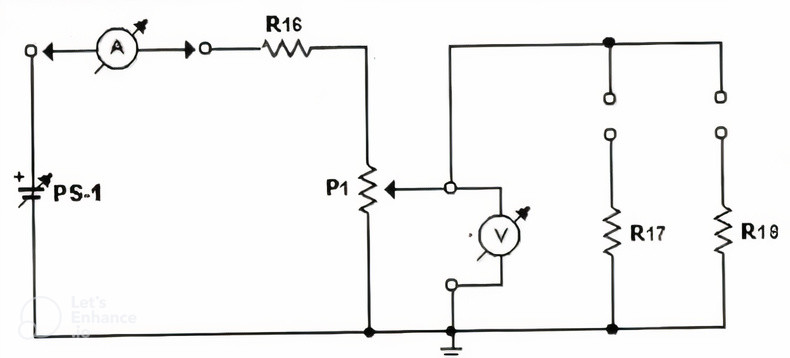
\includegraphics[scale=0.5]{imagenes/1}
		\caption{Circuito a evaluar}
	\end{figure}
	\begin{enumerate}
		\item En el circuito anterior, la tensión en el cursor es de 0v.
		\item Se asumiendo que $PS_1 = 12v, R_{6}= 2.2k\Omega, P_{1}= 4.7k\Omega$. El posible rango de tensiones en el cursor es de 0v a 8.17v. 
	\end{enumerate}
\end{enumerate}
\section{Equipo}
El siguiente equipo es necesario para la realización de la experiencia:
\begin{enumerate}
	\item Módulo de experimentación.
	\item DMM (Multímetro digital).
\end{enumerate}
\section{Procedimiento}
\begin{enumerate}
	\item Mida y registre la resistencia total del potenciómetro.
	\\ $R_{total}= 0.0003K\Omega$
	\item Estudie el siguiente circuito
	
	\begin{figure}[h]
		\centering
		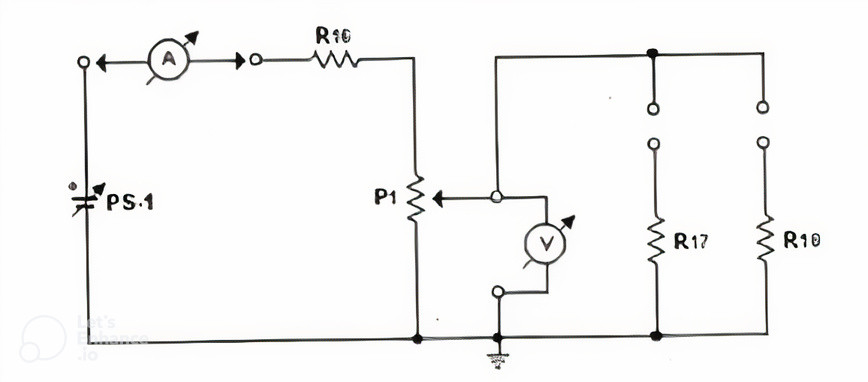
\includegraphics[scale=0.30]{imagenes/2}
		\caption{Segundo circuito}
	\end{figure}
	\item Gire el potenciómetro a fondo en sentido antihorario, y gire luego el dial en sentido horario un $20\%$ de su capacidad de rotación. Mida la resistencia entre el cursor y masa.
	\\ R=8.86K$\Omega$
	\item Conecte la fuente de alimentación $PS-1$ al potenciómetro del modo mostrado en la figura 3.
	\item Lleve  $PS-1$ a $6v$. Mida las tensiones en vació y con las cargas $R_{7}$ y $R_{8}$ respectivamente.
	\begin{table}[h]
		\centering
		\begin{tabular}{|c|c|c|c|c|}
			\hline
			\textbf{Rotación ($\%$)}&\textbf{Resistencia $\Omega$}&\textbf{$V_{sal}$}&\textbf{$V_{sal} R_{17 carga}$}&\textbf{$V_{sal} R_{18 carga}$}\\
			\hline 
			$20\%$&8.87K$\Omega$&0.2&0.2&0.2\\ 
			\hline 
			$40\%$&6.99k$\Omega$&0.56&0.56&0.56\\ 
			\hline
			$60\%$&4.90k$\Omega$&1.5&1.5&1.5\\ 
			\hline
			$80\%$&2.57k$\Omega$&1.67&1.67&1.67\\ 
			\hline
			$100\%$&0.0001k$\Omega$&2.42&2.42&2.42\\ 
			\hline
		\end{tabular}
		\caption{}
	\end{table}
	\item Mida la tensión de salida entre el cursor y masa.
	\item Conecte $R_{17}$ al cursor y  mida las tensiones.
	\item Reemplace $R_{17}$ con $R_{18}$.
	\item Repita este procedimiento para rotaciones de $40\%, 60\%, 80\%$ y $100\%$. La resistencia del potenciómetro debería ser.
	\\
	\textbf{$\% Rotación \frac{+}{-} Resistencia Total$}
	\\
	Siga este procedimiento:
	\begin{enumerate}
		\item Desconecte $PS-1$, Mida la resistencia del potenciómetro con un ohmímetro y anótela.
		\item Vuelva a conectar $PS-1$, mida y anote $V_{sal}$ sin carga.
		\item Conecte $R_{17}$. Mida y anote $v_{sal}$.
		\item Conecte $R_{18}$ de $R_{17}$, mida y anote $v_{sal}$.
	\end{enumerate}
	\begin{table}[h]
		\centering
		\begin{tabular}{|c|c|c|c|c|}
			\hline
			\textbf{Rotación ($\%$)}&\textbf{Resistencia $\Omega$}&\textbf{$V_{sal}$}&\textbf{$V_{sal} R_{17 carga}$}&\textbf{$V_{sal} R_{18 carga}$}\\
			\hline 
			$20\%$&8.86K$\Omega$&0.21&0.21&0.21\\ 
			\hline 
			$40\%$&6.98k$\Omega$&0.60&0.60&0.59\\ 
			\hline
			$60\%$&4.88k$\Omega$&1.17&1.17&1.15\\ 
			\hline
			$80\%$&2.55k$\Omega$&1.91&1.91&1.86\\ 
			\hline
			$100\%$&0.0001k$\Omega$&2.481&2.81&2.77\\ 
			\hline
		\end{tabular}
		\caption{}
	\end{table}
	\item Construya un gráfico de $v_{sal}$ medida (en el eje vertical) en función del porcentaje de rotación (en el eje horizontal) para las tres condiciones de carga.
	\\
	\\
	\\
	\\
	\\
	\\
	\begin{figure}[h]
		\centering
		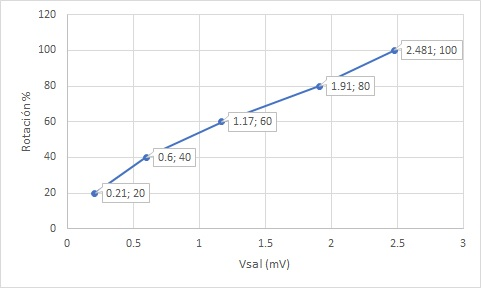
\includegraphics[scale = 0.75]{imagenes/10.1}
		\caption{$V_{sal}$ del potenciómetro}
	\end{figure}
	\begin{figure}[h]
		\centering
		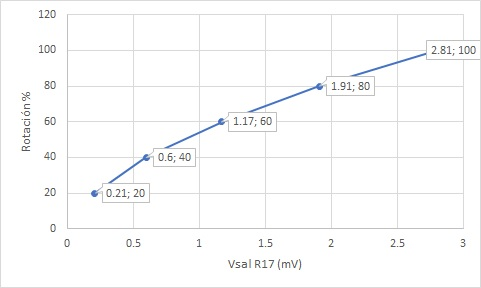
\includegraphics[scale = 0.75]{imagenes/10.2}
		\caption{$V_{sal}$ de $R_{17}$}
	\end{figure}
	\begin{figure}[h]
		\centering
		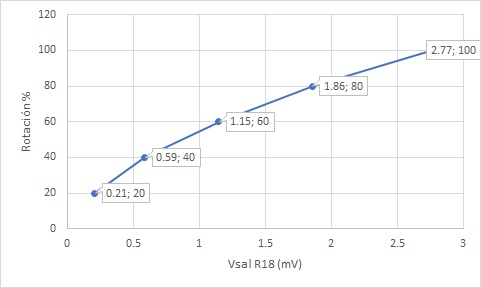
\includegraphics[scale = 0.75]{imagenes/10.3}
		\caption{$V_{sal}$ de $R_{18}$}
	\end{figure}
\end{enumerate}
\section{Autoevaluación}
Estas preguntas probarán su conocimiento sobre el potenciómetro. Evalué el circuito del potenciómetro.
\\
\begin{figure}[h]
	\centering
	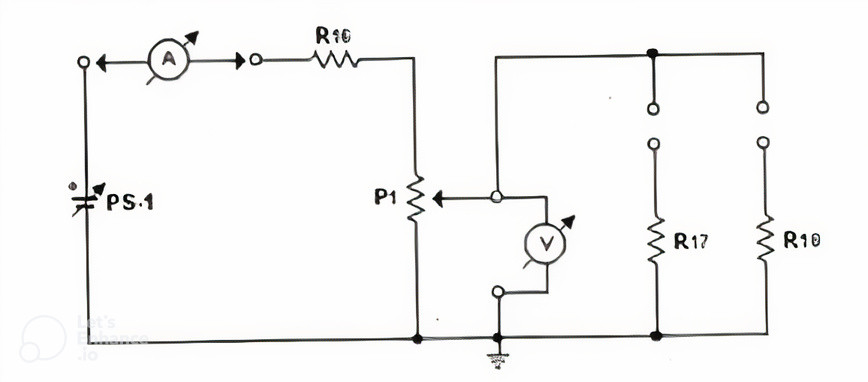
\includegraphics[scale=0.3]{imagenes/2}
	\caption{Circuito a evaluar}
\end{figure}
\begin{enumerate}
	\item Cargar la salida del potenciómetro qué efecto tiene sobre la salida la resistencia aumenta a su valor máximo y lo impide pasar la corriente así generando la caída de tensión en el circuito.
	\item Al aumentar el valor de la resistencia de carga disminuye el voltaje de acuerdo va subiendo el valor de la resistencia.
	\item Suponga que $Ps-1 =12v, R_{16}= 27k\Omega, P_{1}= 10k\Omega$ y $R_{17}=47k\Omega$ están conectados. El rango de la tensión de salida es de 0v a 7.64v. 
	\item Suponga que $Ps-1 =12v, R_{16}= 27k\Omega, P_{1}= 10k\Omega$ y $R_{17}=47k\Omega$ están conectados. La tensión de salida es al $50\%$ es de 3.06v.  
	\item Suponga que $Ps-1 =12v, R_{16}= 27k\Omega, P_{1}= 10k\Omega$ y $R_{17}=47k\Omega$ están conectados. Cuando el potenciómetro es rotado a la posición de $60\%$, la tensión de salida es de 3.84v.
\end{enumerate}
\section{Conclusión}
En este la laboratorio se llego a conocer como es el funcionamiento de un potenciómetro, que efectos produce en las resistencias restantes que se encuentran el circuito. Al girar el dial del potenciómetro la resistencia puede aumentar o disminuir de acuerdo al sentido del giro. Los giros pueden ser de manera horaria o antihoraria. Si el giro es horario la resistencia aumenta hasta llegar a u valor máximo, y si se gira de manera antihoraria la resistencia sera $0\Omega$.